\documentclass[12pt,legal]{article}

\usepackage[margin=1in]{geometry}
\usepackage{titlesec}
\usepackage{tikz}

\usetikzlibrary{shapes.geometric, arrows}

\tikzstyle{startstop} = [rectangle, rounded corners, minimum width=3cm, minimum height=1cm,text centered, draw=black, fill=red!30]
\tikzstyle{io} = [trapezium, trapezium left angle=70, trapezium right angle=110,
minimum width=3cm, minimum height=1cm, text centered, draw=black, fill=blue!30]
\tikzstyle{process} = [rectangle, minimum width=3cm, minimum height=1cm, text
centered, text width=3cm, draw=black, fill=orange!30]
\tikzstyle{decision} = [diamond, minimum width=3cm, minimum height=1cm, text centered, draw=black, fill=green!30]
\tikzstyle{arrow} = [thick,->,>=stealth]

\usepackage{listings}
\usepackage{color}

\titleformat{\section}
{\Large\bfseries}
{}
{0em}
{}[\titlerule]

\titleformat{\subsection}
{\bfseries\small}
{}
{0em}
{}

\begin{document}

\section{Mount Kenya University}
\subsection{BIT 1102: Introduction to Computer Programming and Algorithm CAT1}
\subsection{Name: Wilfred Githuka Reg.Number: BIT2019/44664}

Question1:(a) Description of 3 control structures that make up a computer program.
\begin{enumerate}
  \item{Sequence - In sequence, program statements are executed in the sequence
      in which they appear in the proram}
  \item{Selection or Descision - It gives a choice such that if an expression
      is related to a specific statement its executed, otherwise it is skipped.}
  \item{Iteration or Looping - A group of statements in a program may have to
        be executed repeatedly until some condition is satisfied. This is known
        as looping.}
  \end{enumerate}
Question1:(b) Explanation of a good program
    \begin{enumerate}
    \item{Portability: This is the ability of a program or application to run on
        different platforms (OSs) with or without minimal changes}
      \item{Readability: The program should be written in such a way that it
          makes other programmers or users to follow the logic of the program
          without much effort}
      \end{enumerate}
Question1:(c) FlowChart and Pseudocode for KK Security Ltd Wages
Calculation.
\begin{itemize}
\item{Weekly wage = 5 days}
\item{Daily wage = 8hrs@Ksh320/day for 5 days}
\item{Saturday = 15\% more than weekly wage}
\item{Sunday = 20\% more than weekly wage}
\end{itemize}

\textbf{Pseudocode}

START

DAILY WAGE = 8HRSX320KSH/DAY = 2,360

SATURDAY WAGE = (15\% OF DAILY WAGE) = 382.5

SATURDAY WAGE = (20\% OF DAILY WAGE) = 510

TOTAL WAGE = KSH 3,485.5

STOP


\textbf{Flowchart}

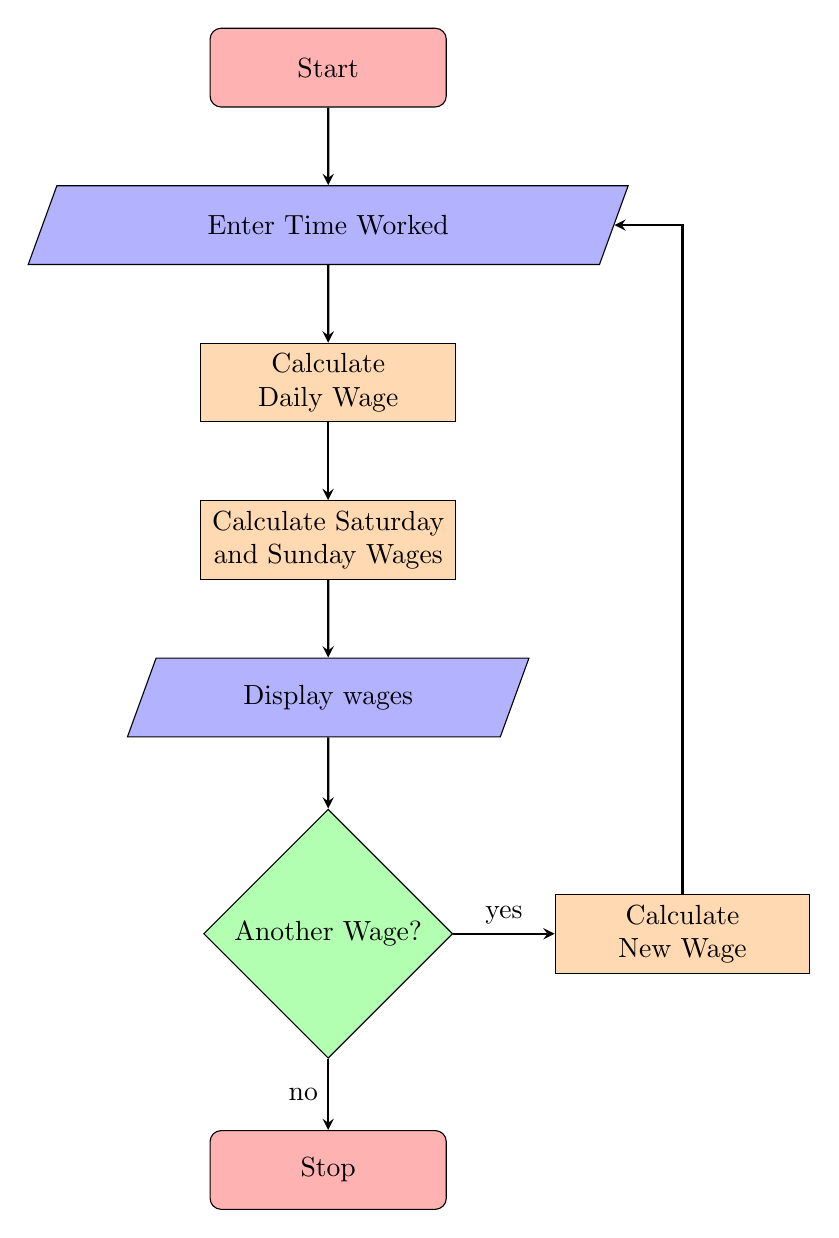
\begin{tikzpicture}[node distance=2cm]
  \node (start) [startstop] {Start};
  \node (in1) [io, below of=start] {Enter Time Worked};
  %\node (pro3) [process, right of=in1, xshift=2cm] {Process 3b};
  \node (pro1) [process, below of=in1] {Calculate Daily Wage};
  \node (pro2) [process, below of=pro1] {Calculate Saturday and Sunday Wages};
  \node (out1) [io, below of=pro2] {Display wages};
  \node (dec1) [decision, below of=out1, yshift =-1cm] {Another Wage?};
  \node (pro2b) [process, right of=dec1, xshift=2.5cm] {Calculate New Wage};
  \node (stop) [startstop, below of=dec1, yshift =-1cm] {Stop};

  \draw [arrow] (start) -- (in1);
  \draw [arrow] (in1) -- (pro1);
  \draw [arrow] (pro1) -- (pro2);
  \draw [arrow] (pro2) -- (out1);
  \draw [arrow] (out1) -- (dec1);
  \draw [arrow] (dec1) -- node [anchor=south] {yes} (pro2b);
  %\draw [arrow] (pro2b) -- (pro3);
  %\draw [arrow] (pro3) -- (in1);
  \draw [arrow] (dec1) -- node [anchor=east] {no} (stop);
  \draw [arrow] (pro2b) |- (in1);
\end{tikzpicture}

Question 2(a) Difference between Pseudocode and Flowchart

A pseudo code is normaly a mixure of English like statements and some
mathematical-like notations and select key words from a programming language.

A flowchart on the other hand, is a diagramatic representations of boxes and
shapes to indicate the flow of logic which is also enhanced by arrows.

Question 2(b) Algorithm and Pseudocode

area = lenth x width

START

INPUT LENGTH

INPUT WIDTH

AREA = LENGTH X WIDTH

END

Question 2(c) Main Ojectives of Programming
\begin{enumerate}
  \item{Problem Solving - Programming is all about solving a problem.
      Programming is the process of developing a program to solve a problem.}
    \item{Maintenance of a program. For an already developed program,
        programming can be applied to make the program better or remove errors.}
      \item{Efficiency - Programming helps in providing code that makes our
          proceses simple, by enabling the computer to do more mudane and
          repetitive tasks.}
        \item{Increase Knowledge - Programming is the process of developing
            software which in itself is a skill that enables us to make more
            products.}
        \end{enumerate}
Question 3(a) Explanation of the characteristics of a good algorithim

\begin{enumerate}
  \item{Each step of an algorithim must be exact. An algorithim must be precise
      and unambigously described.}
    \item{An algorithim must terminate. Since the purpose of an algorithim is to
      solve a problem, if the algorithim does not stop when executed, no output
      shall be gotten from it.}
    \item{An algorithim must be effective. It must provide the correct answer to
      the problem.}  
\end{enumerate}

Question 3(b) Explanation why I would choose a high level lanuage over other
languages.

\begin{itemize}
  \item{High level languages are procedural oriented lanuages and are machine
      independent.}
  \item{High level lanuages are easier to learn than assembly languages}
  \item{High level languages provide better documentation}
  \item{High level languages are easer to maintain}
    \item{High level languages have an extensive vocabulary}
  \end{itemize}

Question 3(c): Structure of a C Program.

%\lstset{language=C}          % Set your language (you can change the language for each code-block optionally)

\lstdefinestyle{customc}{
  belowcaptionskip=1\baselineskip,
  breaklines=true,
  frame=L,
  xleftmargin=\parindent,
  language=C,
  showstringspaces=false,
  basicstyle=\footnotesize\ttfamily,
  keywordstyle=\bfseries\color{green!40!black},
  commentstyle=\itshape\color{purple!40!black},
  identifierstyle=\color{blue},
  stringstyle=\color{orange},
}

\lstdefinestyle{customasm}{
  belowcaptionskip=1\baselineskip,
  frame=L,
  xleftmargin=\parindent,
  language=[x86masm]Assembler,
  basicstyle=\footnotesize\ttfamily,
  commentstyle=\itshape\color{purple!40!black},
}

\lstset{escapechar=@,style=customc}
%\lstset{language=C,caption={Descriptive Caption Text},label=DescriptiveLabel}


 \begin{lstlisting}
#include <stdio.h>

/* This is a Block
 * comment */

int main()
{
    int i;

    // Thi is a line comment.
    printf("Hello world!");
    
    for (i = 0; i < N; i++)
    {
        printf("C is great for programmers!");
    }

    return 0;
  }
\end{lstlisting}

  Every C program contains a function called main main. This is the start point
  of the program.

  The stdio.h allows the program to interact with the screen, keyboard and
  file  system of your computer.

  main() declares the start of the function, while the two curly brackets show
  the start and  finish of the function mostly the body of the function.

  Inside the main function is where the body of the program lies, and what is
  inside it shall be executed when the program is running.

  printf is the printing function that will output text given to it.

  
 
\end{document}
